Recapitulando, en la aproximación lineal, las ecuaciones MHD permiten
la presencia de ondas Alfv\'en. El caso más simple corresponde a MHD
incompresible con un campo magnético de fondo uniforme $\vec{B}_0$,
para el cual la relación de dispersión lineal (en el caso ideal no
disipativo) describe ondas con frecuencia $ \omega =
\vec{k}\cdot\vec{V}_A$, para el número de onda $\vec{k}$, velocidad de
Alfv\'en $\vec{V}_A = \vec{B}_0 / \sqrt{4\pi\rho}$, y densidad
$\rho$. Además, las componentes de Fourier complejas de la velocidad
$\vec{v}(\vec{k})$ y de las fluctuaciones del campo magnético
$\vec{b}(\vec{k})$ son transversales al vector de onda, es decir,
$\vec{v}(\vec{k}) \cdot \vec{k} = \vec{b}(\vec{k}) \cdot \vec{k} =
0$. Curiosamente, estas ondas cuando se consideran de forma aislada
son soluciones no lineales exactas de las ecuaciones MHD.

Sin embargo, cuando se tienen en cuenta los términos no lineales, el
sistema también puede desarrollarse lejos de la dinámica de
equilibrio, con las ondas coexistiendo con remolinos en un flujo
turbulento completamente desarrollado [\cite{dmitruk_waves_2009}].  En
este régimen turbulento, no es necesariamente esperable una relación
directa o explícita entre la frecuencia y el número de onda, tal como
una relación de dispersión de las ondas.  Este régimen está
caracterizado por interacciones de distintos tipos, tales como
distorsiones no lineales, locales en escala, de los \textit{eddies}
[\cite{monin_statistical_2013, kolmogorov_local_1941,
    mccomb_physics_1992}], y efectos no locales
[\cite{alexakis_turbulent_2007, alexakis_anisotropic_2007,
    teaca_energy_2009, mininni_scale_2011}], donde el más extremo es
el \textit{sweeping} de las pequeñas escalas por los grandes
\textit{eddies} [\cite{kraichnan_structure_1959,
    tennekes_eulerian_1975, chen_sweeping_1989, nelkin_time_1990}].
Como ya vimos, para turbulencia MHD [\cite{pouquet_strong_1976,
    zhou_magnetohydrodynamic_2004}], adicionalmente al tiempo no
lineal global $\tau_{nl}$, hay también otras escalas temporales
asociadas a efectos no lineales dependientes de escala (local),
\textit{sweeping} y propagación de ondas.

%% {\color{purple} Al comienzo de la década de 1970, la investigación de la turbulencia
%% hidrodinámica se dirigió al estudio del tiempo de descorrelación del
%% campo de velocidades [\cite{orszag_numerical_1972,
%% orszag_analytical_1970, tennekes_eulerian_1975, heisenberg_zur_1948,
%% comte-bellot_simple_1971}]. La conclusión principal fue que el
%% \textit{sweeping} domina la descorrelación temporal en el rango
%% inercial [\cite{zhou_non-gaussian_1993,sanada_random_1992}].
%% Recientemente, se realizó un estudio similar para magnetohidrodinámica
%% [\cite{servidio_time_2011, matthaeus_eulerian_2010,
%% carbone_anisotropy_2011}]. Una diferencia con el caso hidrodinámico es
%% la presencia de otros fenómenos no locales (además del barrido), como
%% la propagación Alfv\'enica o la distorsión Alfv\'enica, a saber, el
%% ``barrido magnético''. El resultado principal de 
%% \cite{servidio_time_2011} respecto de la descorrelación temporal para
%% turbulencia isotrópica fue que, como en hidrodinámica, la
%% descorrelación temporal en MHD es gobernada por interacciones no
%% locales (en este caso, \textit{sweeping} y descorrelación de
%% Alfv\'en). Sin embargo, no pudieron distinguir entre los efectos del
%% \textit{sweeping} y de la distorsión Alfv\'enica.} MOVIDO A \cref{sec2:SpectraFreq}

En este capítulo, nuestro objetivo será profundizar el análisis
iniciado por \cite{servidio_time_2011} (ver
sección \ref{sec2:SpectraFreq}) y generalizarlo a plasmas magnetizados
a grandes escalas, donde la aproximación MHD resulta válida. Para
ello, estudiaremos los diferentes tiempos de correlación que aparecen
para las distintas escalas en el rango inercial de turbulencia MHD con
un campo guía. El objetivo principal será entender la descorrelación
temporal de las fluctuaciones, estudiando el valor relativo de los
tiempos de descorrelación para diferentes escalas. Así, seremos
capaces de relacionar las leyes de escalas de los tiempos de
descorrelación con la contribución de los diferentes efectos físicos:
distorsión no lineal, \textit{sweeping} aleatorio y propagación de
ondas de Alfv\'en. En otras palabras, estudiaremos la memoria
característica para cada escala espacial, a fin de identificar los
mecanismos de descorrelación temporal y observar si son locales o
no. Con este objetivo, consideraremos las fluctuaciones a más de una
escala espacial, para discernir entre los diferentes fenómenos
asociados con la descorrelación temporal, en particular la propagación
de ondas de Alf\'en y el \textit{sweeping} aleatorio.  Este método,
basado en el cómputo de espectros espacio-temporales y en las
funciones de correlación, fue propuesto e implementado en fluidos
rotantes por
\cite{clark_di_leoni_quantification_2014} (ver también
\cite{clark_di_leoni_spatio-temporal_2015} para una descripción
general del método). Meyrand y Galtier recientemente utilizaron el
espectro espacio-temporal para estudiar la transición de turbulencia
débil a turbulencia fuerte en MHD [\cite{meyrand_direct_2016}], y la
intermitencia en turbulencia MHD débil
[\cite{meyrand_weak_2015}]. Aquí consideramos el régimen de
turbulencia fuerte, y computamos tanto los espectros como los tiempos
de descorrelación.

La estructura del capítulo será la siguiente. En
la sección \ref{sec3:EqNumSim} introduciremos las ecuaciones y los métodos
numéricos empleados, así como también una descripción del espectro
espacio-temporal y de las funciones de correlación. Luego, en
la sección \ref{sec3:Res} presentaremos los resultados. Finalmente, la
discusión y las conclusiones serán expuestas en
la sección \ref{sec3:Conclusions}.

%%%%%%%%%%%%%%%%%%%%%%%%%%%%%%%%%%%%%%%%%
\section{Ecuaciones y simulaciones numéricas}\label{sec3:EqNumSim}

\subsection{Las ecuaciones MHD}\label{sec3:eq}

Las \cref{eq2:NS-MHDv,eq2:NS-MHDB} de MHD incompresible pueden
adimensionalizarse, obteniendo
\begin{equation}\label{eq3:MHD_v}
  \frac {\partial \vec{v}}{\partial t} +
  \vec{v }\cdot \nabla \vec{v} = -\frac{1}{\rho}\nabla p +
  \vec{j} \times \vec{B} + \frac{1}{R} \nabla^2\vec{v} + \vec{F}_v,
\end{equation}
\begin{equation}\label{eq3:MHD_b}
  \frac{\partial \vec{b}}{\partial t} = \nabla \times (\vec{v} \times \vec{B})
  + \frac{1}{R_m} \nabla^2 \vec{b} + \vec{F}_b,
\end{equation}
donde $\vec{v}$ es la velocidad del plasma; $\vec{B} = \vec{b}
+ \vec{B}_0$ el campo magnético, con una parte fluctuante $\vec{b}$ y
un campo medio DC $\vec{B_0}=B_0\hat{x}$; $\vec{j}
= \nabla \times \vec{b}$ la densidad de corriente; $p$ la presión,
$\rho$ la densidad del plasma, y $\vec{F}_v$ y $\vec{F}_b$ términos de
forzado que luego serán discutidos con más detalles. Las unidades se
basan en una velocidad característica $v_0$, que para MHD se toma como
la velocidad de Alfvén típica de las fluctuaciones del campo
magnético, $v_0 = \sqrt{\langle b^2 \rangle /(4\pi\rho)}$, con
$\langle . \rangle$ el promedio espacial. Los parámetros
adimensionales que aparecen en las ecuaciones son los números de
Reynolds cinético y magnético, es decir $R=v_0 L/\nu$ y $R_m = v_0 L
/\mu$, respectivamente, con $\nu$ la viscosidad cinemática, $\mu$ la
difusividad magnética y $L$ una escala de longitudes característica
(la caja de la simulación tiene un tamaño dado de $2\pi L$). La unidad
temporal es $t_0 = L/v_0$, que para MHD se convierte en el tiempo de
cruce Alfv\'enico (\emph{Alfv\'en crossing time}) basado en las
fluctuaciones del campo magnético.


\subsection{Espectros y funciones de correlación}\label{sec3:Wfspectrum_and_Gamma}

A partir de las ecuaciones \cref{eq3:MHD_v,eq3:MHD_b} y argumentos de
escala, es posible estimar los diferentes tiempos característicos. El
tiempo de los \textit{eddy turnover} locales puede ser definido como
$\tau_{nl} \sim \left[ k v(k) \right]^{-1}$, donde $k$ es el número de
onda y $v(k)$, la amplitud de la velocidad debido a las fluctuaciones
a escala $\sim 1/k$. Para una predicción del escaleo de velocidades
tipo Kolmogorov, $v \sim v_{rms} \left(kL\right)^{-1/3}$, las escalas
de tiempo no lineal en el rango inercial pueden ser escritas
aproximadamente como
\begin{equation}
\tau_{nl} = C_{nl} \left [
   v_{rms} L^{-1/3} \left(\sqrt{k^2_\perp +
   k^2_\parallel}\right)^{2/3}\right ]^{-1},
\label{eq3:taunl}
\end{equation}
donde $C_{nl}$ es una constante adimensional del orden de la
unidad (para una discusión más detallada,
ver \cite{zhou_magnetohydrodynamic_2004}). En lo que sigue, $v_{rms}
= \left\langle |\vec{v}|^2 \right\rangle ^{1/2}$ es una cantidad
global, típicamente dominada por las contribuciones de las grandes
escalas.

La física de la descorrelación temporal depende de otros efectos y,
por lo tanto, de otras escalas de tiempo MHD disponibles. Un ejemplo
es el tiempo característico de barrido a escala $\sim 1/k$, que puede
expresarse como
\begin{equation}
\tau_{sw} = C_{sw} \left( v_{rms}\sqrt{k^2_\perp + k^2_\parallel}
    \right)^{-1}.
\label{eq3:tausw}
\end{equation}
Este tiempo corresponde a la advección
de estructuras a pequeña escala por el flujo a gran
escala. Análogamente, se puede definir un tiempo de Alfvén
característico como
\begin{equation}
\tau_A= C_A \left( v_A k_\parallel \right)^{-1}.
\label{eq3:taua}
\end{equation}
Aquí, $C_{sw} $ y $C_A$ son otras constantes adimensionales del
orden de la unidad. Todas estas escalas de tiempo dependen del vector
de onda, y suponiendo que la escala de tiempo más corta domina la
dinámica, se pueden definir diferentes regiones en el espacio
$\vec{k}$ en el espectro de energía.

Las estadísticas de, por ejemplo, el campo magnético, puede ser
caracterizado por la función de correlación a dos puntos
espacio-temporal
\begin{equation}
R(\vec{r},\tau) = \left\langle \vec{b}( \vec{x},t) \cdot
  \vec{b}( \vec{x} + \vec{r},t+\tau) \right\rangle / \left\langle {\bf
    b}^2 \right\rangle.
\label{eq3:Rbij}
\end{equation}
Notar que esta expresión contiene tanto el espectro de energía como el
espectro de frecuencia Euleriano (teorema de Wiener-Khinchin); sin
embargo, contiene mucha más información que nos permite hacer un
análisis más sutil de las relaciones espacio-temporales.
Transformando Fourier en $r$, obtenemos una densidad espectral
retrasada temporalmente, que puede a su vez factorizarse como
$S(\vec{k},\tau) = S(\vec{k})\Gamma(\vec{k},t)$, donde $\vec{k}$ es el
vector de onda. La función $\Gamma(\vec{k},\tau)$, la función de
correlación dependiente de la escala [\cite{heisenberg_zur_1948,
comte-bellot_simple_1971, orszag_numerical_1972}], representa los
efectos dinámicos de descorrelación que describen la descorrelación de
tiempo de cada modo espacial $\vec{k}$.

Entonces, la función $\Gamma(\vec{k},\tau)$ es la función de
correlación temporal del modo de Fourier $\vec{k}$. Usando esto,
seremos capaces de identificar el tiempo de descorrelación
característico para cada modo $\vec{k}$, y en consecuencia la pérdida
de memoria de las fluctuaciones 3D cuyas longitudes características
sean de orden $k_x^{-1}$, $k_y^{-1}$ y $k_z^{-1}$. Cuando no hay campo
guía, es esperable que el flujo sea isotrópico tanto en el espacio
real como en el de Fourier, y en consecuencia es suficiente con
estudiar la función $\Gamma(k,\tau)$, que depende sólo de
$k=|\vec{k}|$. Por otra parte, en presencia de un campo guía la
turbulencia se vuelve anisotrópica; entonces, es razonable usar
$\Gamma = \Gamma(k_\perp,k_\parallel,\tau)$, con $k_\perp$ y
$k_\parallel$ los números de onda de Fourier perpendiculares y
paralelos al campo magnético medio.

La función $\Gamma(k_\perp,k_\parallel,\tau)$ puede ayudarnos a
entender la dinámica en las diferentes regiones del espacio de
Fourier. Por ejemplo, la función $\Gamma(k_\perp=0,k_\parallel,\tau)$
nos da información acerca de las fluctuaciones que varían sólo en la
dirección paralela.  De la misma manera,
$\Gamma(k_\perp,k_\parallel=0,\tau)$ nos da información acerca de las
fluctuaciones que sólo varían en la dirección perpendicular. También
es interesante la información obtenida de
$\Gamma(k_\perp=k_0,k_\parallel,\tau)$ y de
$\Gamma(k_\perp,k_\parallel=k_0,\tau)$, donde uno de los números de
onda (el paralelo o el perpendicular) se deja igual a un valor fijo
$k_0$. Por ejemplo, estudiando el tiempo de descorrelación para
$\Gamma(k_\perp=k_0,k_\parallel,\tau)$ en función de $k_\parallel$
podría ser útil para ver la pérdida de memoria a lo largo del tiempo
de las fluctuaciones cuya longitud característica perpendicular es
$\sim k_0^{-1}$ (a una longitud fija seleccionada), en función de su
escala paralela $\sim k_\parallel^{-1}$. Esto nos da información de
dos cuestiones importantes: cómo la memoria en una dirección afecta la
otra, y más importante, cómo distinguir entre \textit{sweeping}
aleatorio y propagación de Alfvén.


\subsection{Simulaciones numéricas}\label{sec3:NumSim}

Utilizamos un código pseudoespectral estándar para resolver
numéricamente las ecuaciones MHD 3D incompresibles con un campo guía
[\cite{gomez_parallel_2005, gomez_mhd_2005}]. Todos los resultados
reportados aquí corresponden a simulaciones con resoluciones de $N^3 =
512^3$ puntos de grilla. Para la integración temporal, se utilizó un
esquema de Runge-Kutta de segundo orden. Se utilizaron campos
magnéticos guía débiles, moderados y fuertes, $B_0 = 0.25$, $1$ y $8$
(en unidades del valor \textit{r.m.s} inicial de las fluctuaciones
magnéticas). También consideramos el caso $B_0 = 0$ como referencia
con estudios previos [\cite{servidio_time_2011}]. Se tomaron
condiciones de contorno periódicas en todas las direcciones de un cubo
de lado $2\pi L$ (donde $L = 1$ es la longitud de correlación inicial
de las fluctuaciones, definida como la unidad de longitud). Se
removió el \textit{aliasing} mediante el método de truncamiento de la
regla de los dos-tercios. La condición inicial en todas las simulaciones consistió en amplitudes
no nulas para los campos $\vec{v}(\vec{k})$ y $\vec{b}(\vec{k})$,
equiparticionados en todos los números de onda dentro de los
cascarones con $1.1 \leq k \leq 4$ (en unidades de $2\pi L/\lambda$,
con $\lambda$ la longitud de onda). Se eligieron fases aleatorias para
todos los modos de Fourier en ambos campos.

Para mantener al sistema
en un estado turbulento estacionario, aplicamos forzados $\vec{F}_b$ y
$\vec{F}_v$ para $\vec{b}$ y $\vec{v}$, respectivamente, en las
\cref{eq3:MHD_v,eq3:MHD_b}). Los forzados $\vec{F}_b$ y $\vec{F}_v$ se
encuentran limitados a una banda fija de modos de Fourier,
$0.9\leq k \leq 1.8$. El forzado tiene una componente aleatoria y una
coherente temporalmente, con un tiempo de correlación del forzado de
$\tau_f \approx 1$ (del orden de la unidad de tiempo $t_0$), que es
mayor que todos los tiempos característicos definidos en la sección
anterior. 

El rango temporal utilizado para analizar los resultados es de más de
$20$ unidades de tiempo para $B_0=0$ y $B_0=0.25$, más de $25$
unidades temporales para $B_0=1$, y más de $10$ unidades temporales
para $B_0=8$. Todos estos períodos de tiempo se consideraron después
de que el sistema alcanzase un estado estacionario turbulento, y
verificamos que eran suficientes para garantizar la convergencia de
los espectros y las funciones de correlación.


%%%%%%%%%%%%%%%%%%%%%%%%%%%%%%%%%%%%%%%%%%%%
\section{Resultados}\label{sec3:Res}

\subsection{Espectros de energía y escalas temporales dominantes}

El espectro axisimétrico de energía $e(|\vec{k_\perp}| =
\sqrt{k_y^2+k_z^2}, k_\parallel = k_x, t)$, definido como
\begin{equation}\label{eq3:axisymmetric}
\begin{split}  e(k_\perp, k_\parallel, t) = \sum_{\substack{k_\perp \leq |\vec{k}\times\hat{x}| < k_\perp+1 \\ k_\parallel \leq k_x < k_\parallel +1}} |\hat{v}(\vec{k},t)|^2 +|\hat{b}(\vec{k},t)|^2 = \\ = \int \left(|\hat{v}(\vec{k},t)|^2 +|\hat{b}(\vec{k},t)|^2\right) |\vec{k}| \sin \theta_k~d\phi_k,
\end{split}
\end{equation}
provee información acerca de la anisotropía de la turbulencia,
relativa al campo guía [\cite{mininni_isotropization_2012}]. En este
estudio, el campo guía es elegido a lo largo del eje $x$, por lo que
las componentes del vector de onda $k_\parallel$ y $k_\perp$, y los
ángulos polares en el espacio de Fourier $\theta_k$ y $\phi_k$, se
toman relativos a este eje. En otras palabras, en
la \cref{eq3:axisymmetric}, $\theta_k = \arctan(k_\perp/k_\parallel)$
es la co-latitud en el espacio de Fourier con respecto al eje $x$ (es
decir, en la dirección del campo guía), y $\phi_k$ es la longitud con
respecto al eje $y$. La primera expresión que involucra la sumatoria
en la \cref{eq3:axisymmetric} es la definición del espectro de energía
axisimétrico para un espacio de Fourier discreto (i.e., como se usa en
las simulaciones), mientras que la segunda expresión con la integral
corresponde al límite del continuo. En lo que sigue, trataremos ambas
expresiones como equivalentes, reemplazando las integrales por
sumatorias cuando sea requerido por el análisis numérico.

A partir del espectro axisimétrico, uno puede definir el espectro
energético perpendicular reducido y promediado temporalmente
$E(k_\perp)$ [\cite{mininni_isotropization_2012}] como
\begin{equation}\label{eq3:reducedspectrum}
  E\left(k_\perp\right) = \frac{1}{T}\int\int e(|\vec{k_\perp}|,
  k_\parallel, t) \, dk_\parallel~dt,
\end{equation}
donde hemos integrado a lo largo de los números de onda paralelos para
obtener un espectro que depende sólo de $k_\perp$. Equivalentemente, el
espectro energético isotrópico puede ser obtenido de la
\cref{eq3:axisymmetric} integrando sobre $\theta_k$ en el espacio de
Fourier. La \cref{fig3-1:E} muestra el espectro isotrópico de energía
$E(k)$ para la corrida con $B_0=0$, y el espectro energético
perpendicular reducido $E(k_\perp)$ para las corridas con campo guía
no nulo.

\begin{figure}
  \centering
  \includegraphics[width=0.8\columnwidth]{SpatioTemporalSpectra/fig1_E-eps-converted-to.pdf}
  \caption{Espectros energéticos perpendiculares reducidos $E(k_\perp)$ para las
  simulaciones con $B_0=0.25$, $1$, $4$, y $8$, y espectro energético
  isotrópico $E(k)$ para la simulación con $B_0=0$. Se muestra como
  referencia el escaleo de Kolmogorov, $\sim k_\perp^{-5/3}$.}
  \label{fig3-1:E}
\end{figure}


La \cref{fig3-2:isocontourns} muestra los contornos de
$e(k_\perp,k_\parallel)/\sin(\theta_k)$, es decir, el espectro
axisimétrico (promediado temporalmente) para las corridas con $B_0=0$,
$B_0=1$, $B_0=4$ y $B_0=8$. Para el flujo isotrópico ($B_0=0$, ver
\cref{fig3-2:isocontourns}a), los contornos de
$e(k_\perp,k_\parallel)/\sin(\theta_k)$ son círculos, tal como se
esperaba [\cite{mininni_isotropization_2012}]. A medida que la
intensidad del campo guía aumenta, la energía se comienza a concentrar
cerca del eje con$k_\parallel=0$, evidenciando la formación de
estructuras elongadas en la dirección del campo guía (o, en otras
palabras, del relativo decrecimiento de los gradientes paralelos del
campo con respecto a los gradientes perpendiculares).

Los tiempos característicos definidos en la
sección \ref{sec3:Wfspectrum_and_Gamma}, $\tau_A$, $\tau_{sw}$ y
$\tau_{nl}$, dividen el espacio de Fourier en
la \cref{fig3-2:isocontourns} en regiones dependiendo de cómo se
ordenan las escalas temporales:
\begin{equation}\label{eq3:Asw} \tau_A < \tau_{sw} \hspace{0.05cm}
\Rightarrow \hspace{0.05cm} k_\perp <
\left(\sqrt{\left(\frac{B_0}{v_{rms}}\right)^2 \cdot
\left(\frac{C_{sw}}{C_A}\right)^2 - 1} \right) k_\parallel,
\end{equation}
\begin{equation}\label{eq3:Anl} \tau_A < \tau_{nl} \hspace{0.05cm}
\Rightarrow \hspace{0.05cm} k_\perp <
\left(\sqrt{\left(\frac{B_0}{v_{rms}}\right)^3
\left(\frac{C_{nl}}{C_A}\right)^3 Lk_\parallel - 1} \right) 
k_\parallel,
\end{equation}
\begin{equation}\label{eq3:nlsw} \tau_{nl} < \tau_{sw} \hspace{0.05cm}
\Rightarrow \hspace{0.05cm} \left( k_\perp^2 + k_\parallel^2
\right)^{1/6} < \frac{C_{sw}}{C_{nl}L^{1/3}}.
\end{equation}
En la \cref{fig3-2:isocontourns} también se indican las curvas
correspondientes a los modos que satisfacen las relaciones
$\tau_A\lesssim\tau_{sw}$ y $\tau_A\lesssim\tau_{nl}$, para $B_0=1$,
$4$ y $8$ (asumiendo, para dibujar las curvas, que $C_{sw} \approx
C_{nl} \approx C_A \approx 1$; esta elección fue posteriormente
confirmada por el análisis de las funciones de correlación). Debe
mencionarse que la curva $\tau_A\approx\tau_{nl}$ también cumple un
rol muy importante en la teoría de balances críticos
[\cite{sridhar_toward_1994}].

Como puede verse de la \cref{eq3:nlsw}, la región donde
$\tau_{nl}\leq\tau_{sw}$ es un círculo pequeño alrededor del origen,
donde $k_\perp^2 + k_\parallel^2 \leq (C_{sw}/L^{1/3}C_{nl})^6 \approx
1$, y no se puede ver en la figura. Los modos fuera de la región con
$\tau_{nl}<\tau_{sw}$ deberían descorrelacionarse con el tiempo de
\textit{sweeping} o con el tiempo de Alfvén, dependiendo de cuál sea
más rápido. La \cref{eq3:Asw} nos dice que en el área a la izquierda de
la curva $\tau_A\sim\tau_{sw}$ tenemos $\tau_A<\tau_{sw}$, mientras
que la \cref{eq3:Anl} nos dice que en el área a la izquierda de la
curva $\tau_A\sim\tau_{nl}$ tenemos $\tau_A<\tau_{nl}$ (ver
\cref{fig3-2:isocontourns}b). Para el valor más grande de $B_0$
considerado (i.e., la simulación con $B_0=8$), la mayoría de los modos
tienen al periodo de Alfvén como el tiempo más rápido (i.e., la mayor
área en el gráfico se encuentre arriba y a la izquierda de la curva
$\tau_A \sim \tau_{sw}$), a pesar de que una fracción significativa de
la energía en el sistema no esté en estos modos, sino que se
concentran cerca del eje con $k_\parallel = 0$.

\begin{figure*}
  \centering
%  \subfigure[$B_0=0$]{\includegraphics[width=0.45\textwidth]{SpatioTemporalSpectra/fig2_B0-eps-converted-to.pdf}}
%  \subfigure[$B_0=0.25$]{\includegraphics[width=0.45\textwidth]{SpatioTemporalSpectra/fig2_B025-eps-converted-to.pdf}}

%  \subfigure[$B_0=1$]{\includegraphics[width=0.45\textwidth]{SpatioTemporalSpectra/fig2_B1-eps-converted-to.pdf}}
%  \subfigure[$B_0=1$ with explanation]{\includegraphics[width=0.45\textwidth]{SpatioTemporalSpectra/fig2_B1_explanation-eps-converted-to.pdf}}

%  \subfigure[$B_0=4$]{\includegraphics[width=0.45\textwidth]{SpatioTemporalSpectra/fig2_B4-eps-converted-to.pdf}}
%  \subfigure[$B_0=8$]{\includegraphics[width=0.45\textwidth]{SpatioTemporalSpectra/fig2_B8-eps-converted-to.pdf}}
  \subfigure[$B_0=0$]{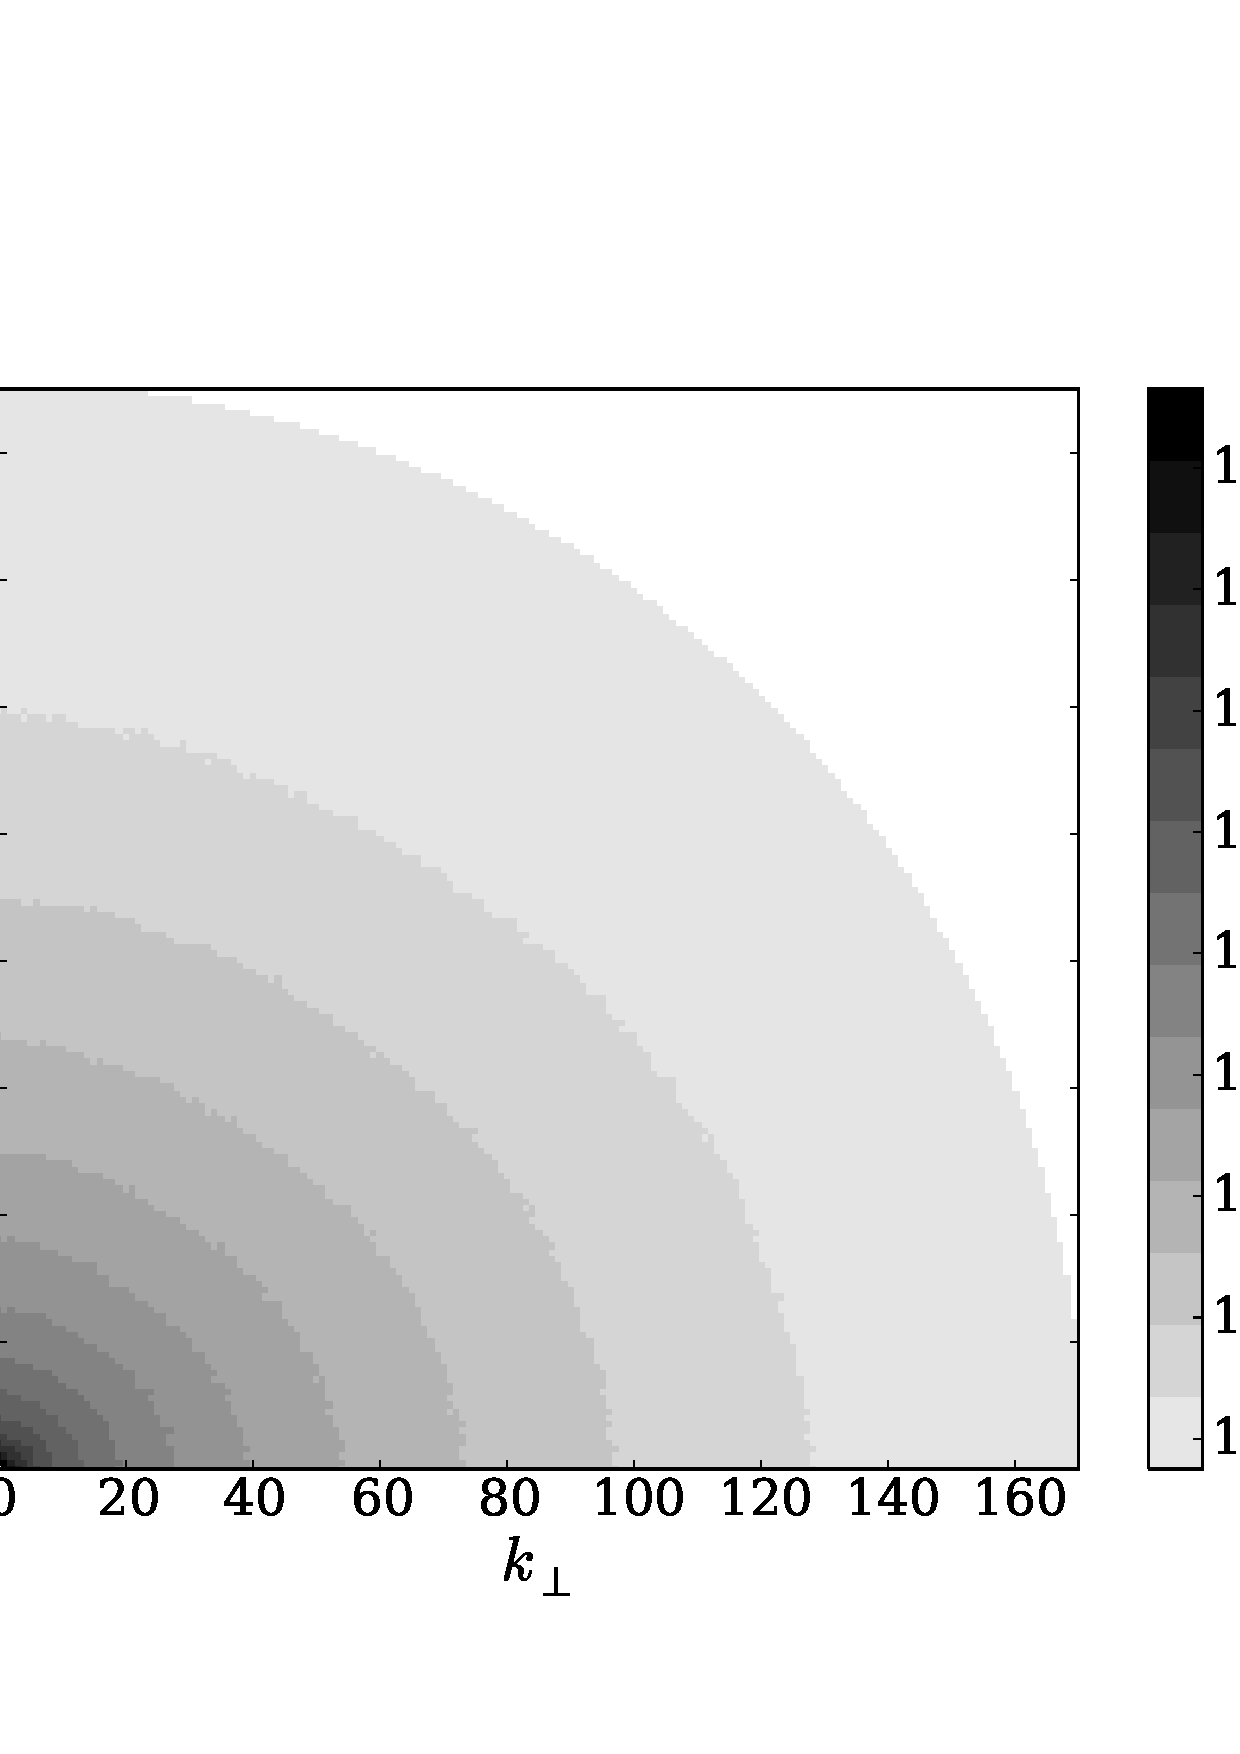
\includegraphics[width=0.48\textwidth]{SpatioTemporalSpectra/fig2_B0.pdf}}\hfill
  \subfigure[$B_0=1$]{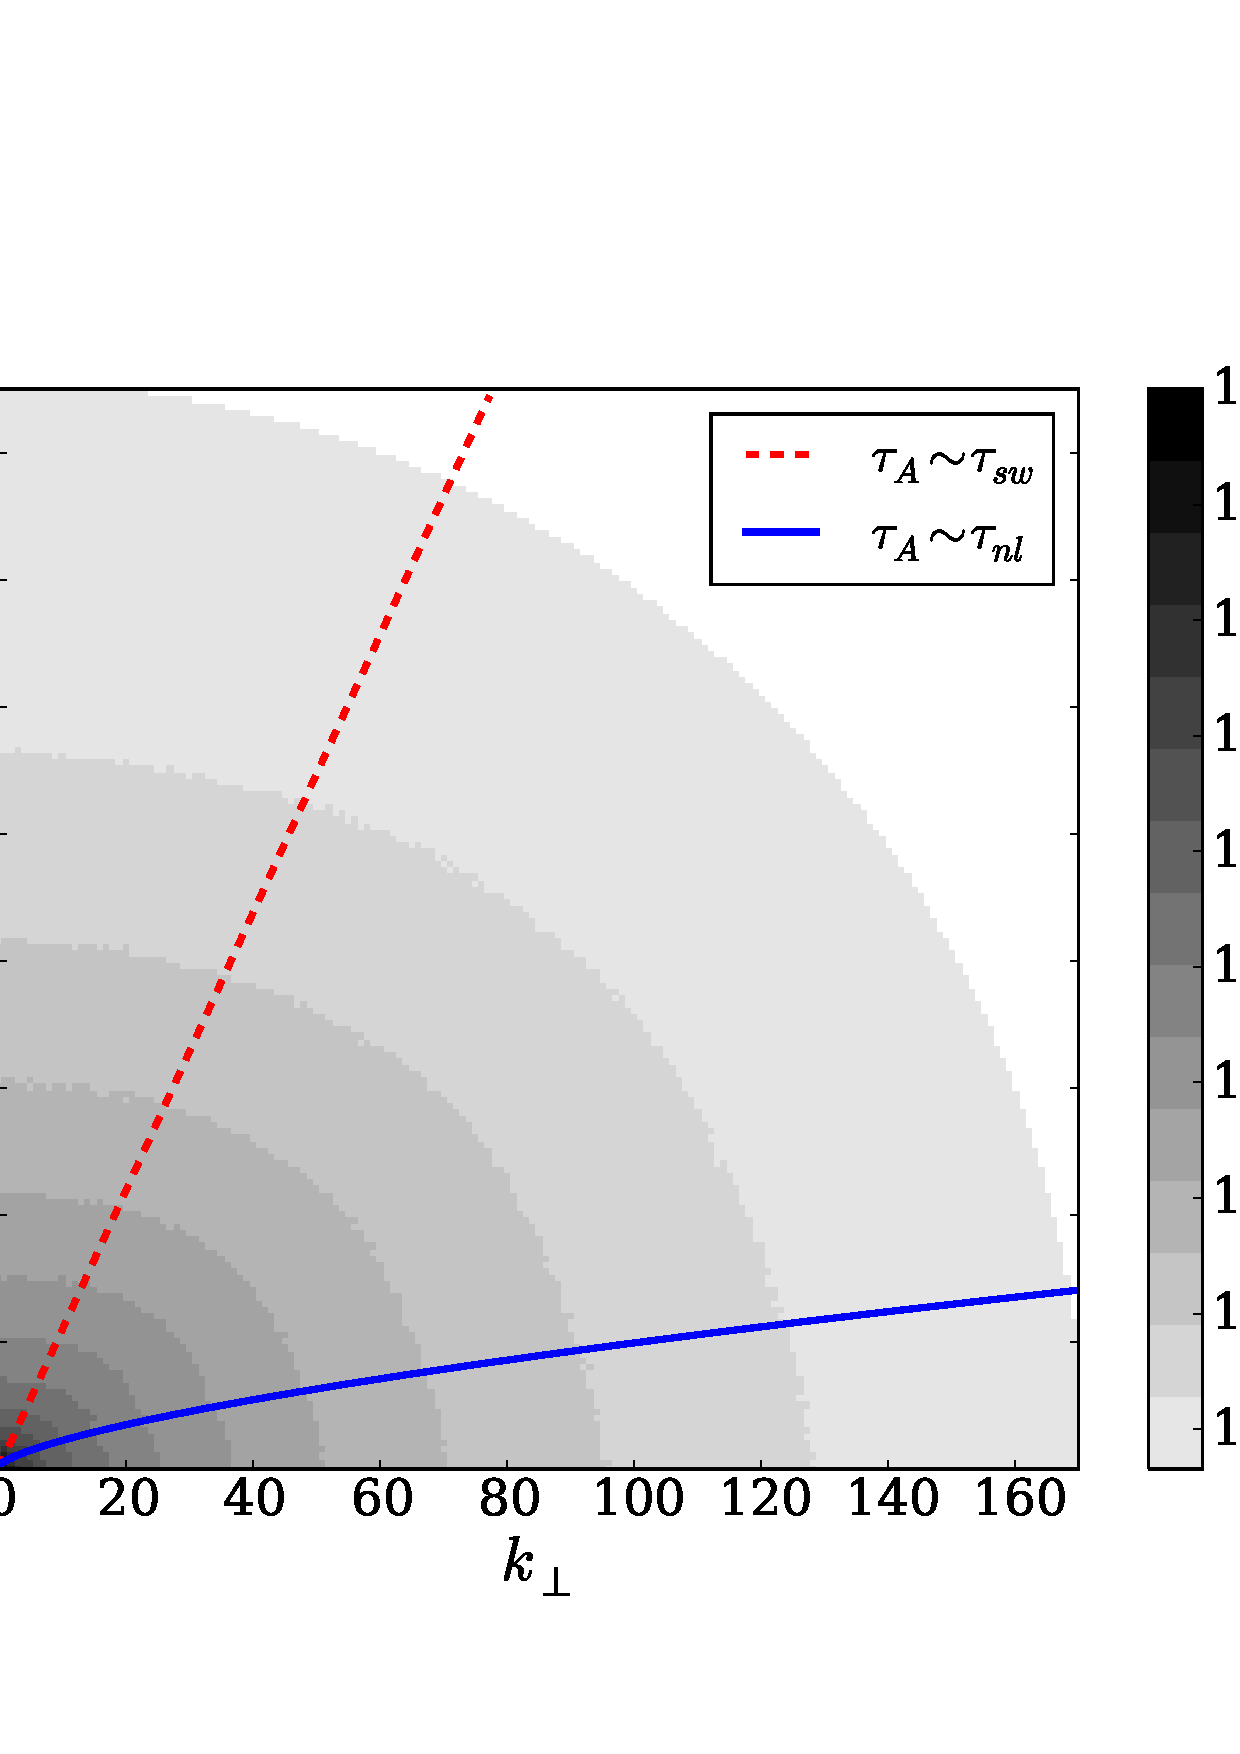
\includegraphics[width=0.48\textwidth]{SpatioTemporalSpectra/fig2_B1.pdf}}

  \subfigure[$B_0=4$]{\includegraphics[width=0.48\textwidth]{SpatioTemporalSpectra/fig2_B4.pdf}}\hfill
  \subfigure[$B_0=4$ en escala doble logaritmo]{\includegraphics[width=0.48\textwidth]{SpatioTemporalSpectra/fig2_B4_log.pdf}}
%  \subfigure[$B_0=4$ in log-log scale]{\includegraphics[width=0.45\textwidth]{SpatioTemporalSpectra/fig2_B4_log.eps}}

  \subfigure[$B_0=8$]{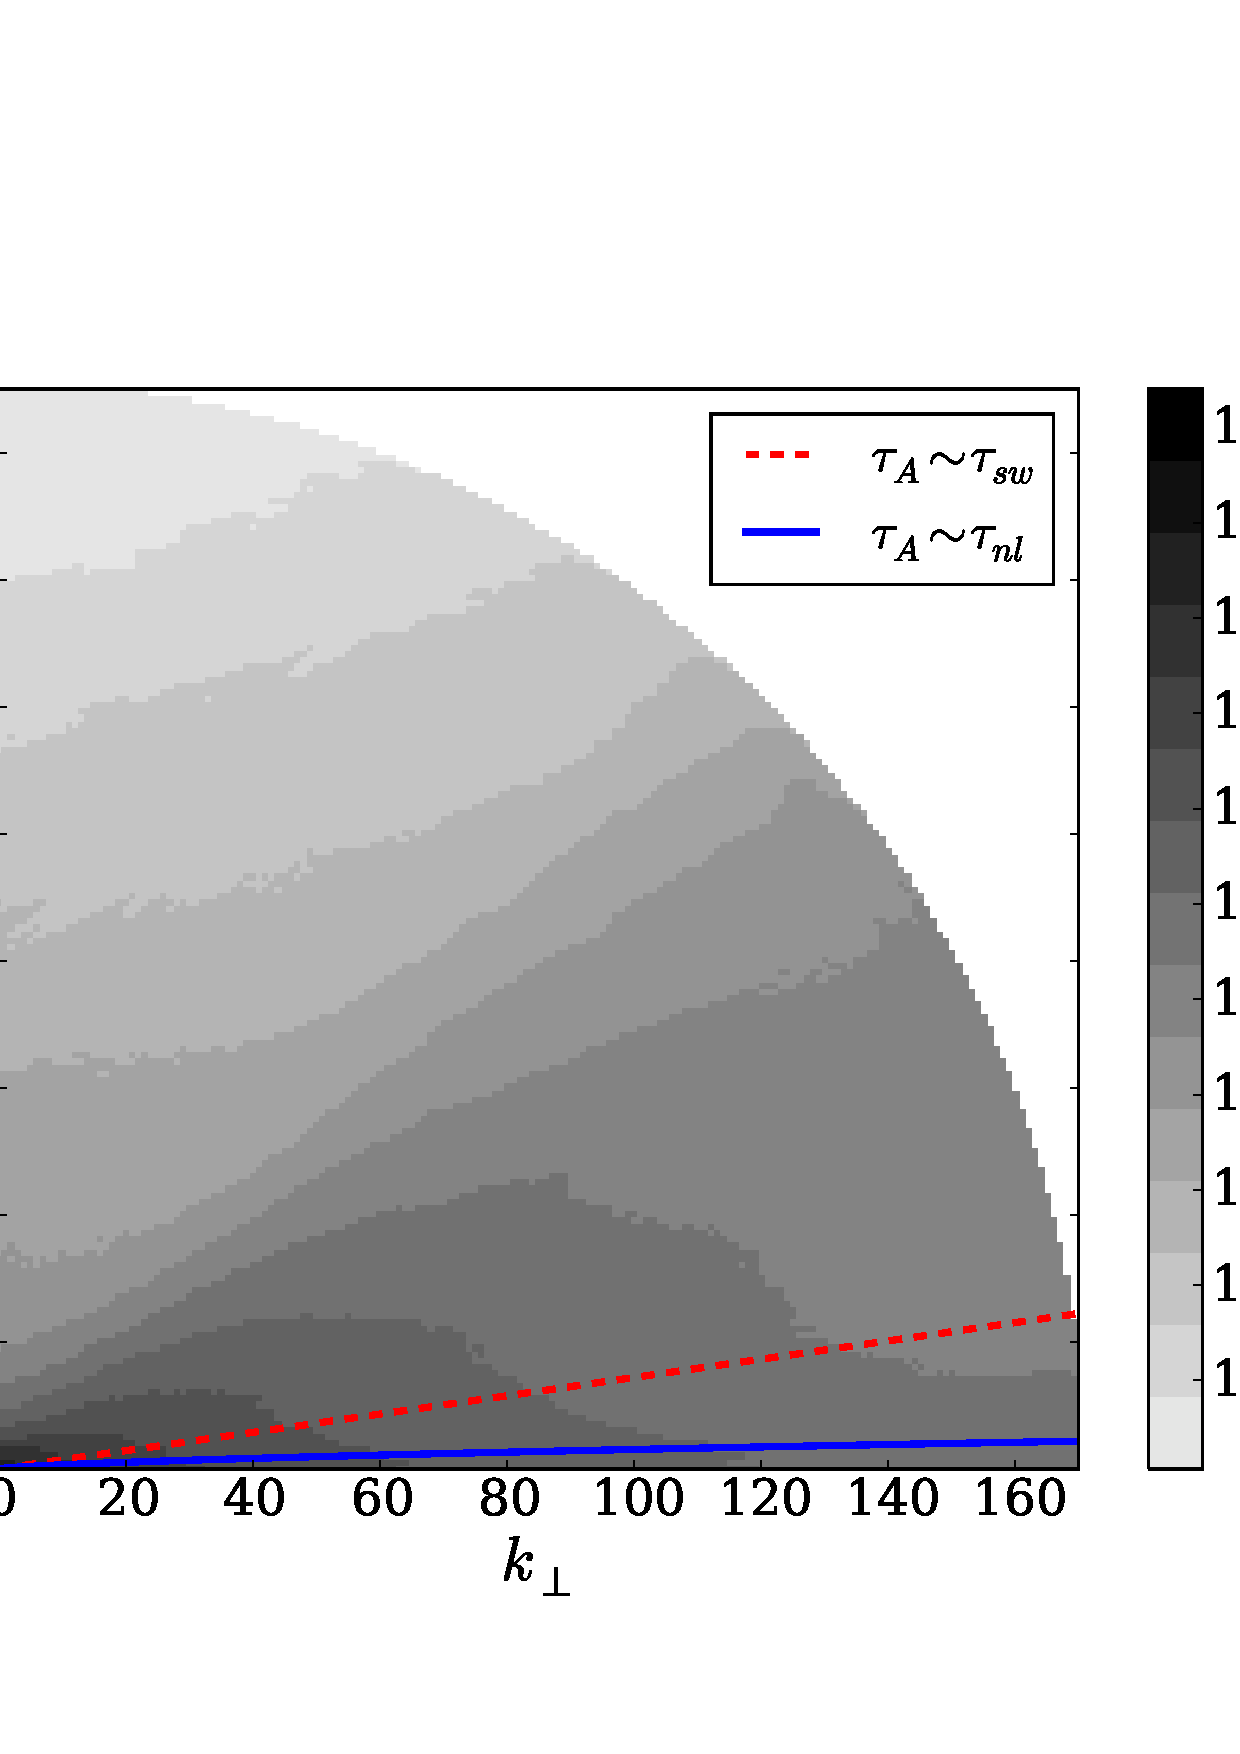
\includegraphics[width=0.48\textwidth]{SpatioTemporalSpectra/fig2_B8.pdf}}\hfill
  \subfigure[$B_0=8$ en escala doble logaritmo]{\includegraphics[width=0.48\textwidth]{SpatioTemporalSpectra/fig2_B8_log.pdf}}
%  \subfigure[$B_0=8$ in log-log scale]{\includegraphics[width=0.45\textwidth]{SpatioTemporalSpectra/fig2_B8_log.eps}}
  \caption{Isocontornos del espectro axisimétrico de energía 
    $e(k_\perp,k_\parallel)$ para $B_0=0$, $1$, $4$ y $8$. Los casos
    con $B_0 = 4$ y $8$ se muestran también en una escala doble logarítmica
    para mostrar con mayor detalle el rango inercial. 
    El color oscuro significa mayor densidad energética (en escala
    logarítmica). Las líneas indican los modos para los que el tiempo de
    \textit{sweeping} o el tiempo no lineal son iguales al tiempo de Alfv\'en.
    Para valores grandes de $B_0$, los isocontornos cambian de forma a
    medida que cruzan cada una de estas líneas. Notar el aumento
    de la anisotropía del espectro a medida que $B_0$ se incrementa, así
    como la mayor superficie cubierta por modos en los que el
    período de Alfv\'en es el tiempo más rápido.}
  \label{fig3-2:isocontourns}
\end{figure*}


\subsection{Espectros espacio-temporales}

Las \cref{fig3-3:B025_bvf_Etot_kperp0,fig3-3:B1_bvf_Etot_kperp0,fig3-3:B8_bvf_Etot_kperp0}
(correspondientes a las simulaciones con $B_0=0.25$, $1$ y $8$,
respectivamente) muestran el espectro en función del vector de onda y
la frecuencia, $E(\vec{k},\omega)/E(\vec{k})$, para modos $\vec{k}$
con $k_\perp = 0$, donde
\begin{equation}
  E(\vec{k})=\int E(\vec{k},\omega)d\omega
\end{equation}
es el espectro de la energía total. Con esta elección para la
normalización, resultan más claramente visibles las frecuencias que
concentran la mayor cantidad de energía para cada $\vec{k}$. Para
$B_0=0.25$ (\cref{fig3-3:B025_bvf_Etot_kperp0}) observamos una clara
dispersión de la energía por debajo de la línea de la relación de
\textit{sweeping} (i.e., vemos excitaciones en todos los modos con frecuencias
iguales o menores que $\omega = v_{rms} k_\parallel$, indicando que
las estructuras de escalas pequeñas están siendo advectadas por todas
las velocidades iguales o menores a $v_{rms}$).  También es observable
para valores pequeños de $k_\parallel$ una acumulación débil cerca de
la relación de dispersión de Alfvén $\omega = B_0 k_\parallel$, aunque
el amplio espectro en el dominio de las frecuencias sugiere que el
\textit{sweeping} es dominante en este caso.

Al incrementar el campo medio a $B_0=1$
(\cref{fig3-3:B1_bvf_Etot_kperp0}), parte de la energía se concentra
por encima de la línea de \textit{sweeping}, y comienza a seguir la
relación de dispersión de Alfvén, aunque el espectro continúa siendo
muy amplio en las frecuencias, con la mayor parte de la energía por
debajo de la relación de \textit{sweeping}.  Este comportamiento
cambia drásticamente para valores más altos de $B_0$.  En
la \cref{fig3-3:B8_bvf_Etot_kperp0} ($B_0=8$), podemos ver que la
energía claramente se concentra alrededor de la relación de dispersión
de las ondas de Alfvén, con un pico de concentración para modos con
hasta $k_\parallel \approx 10$, para posteriormente dispersarse hacia
la relación de \textit{sweeping} para números de onda más grandes.
Notar que este comportamiento indica una competición entre el tiempo
magnetohidrodinámico de \textit{sweeping} y el tiempo de Alfvén, con
este último resultando dominante a grandes escalas para valores de
$B_0$ grandes. Estos resultados respaldan y mejoran los obtenidos por
\cite{dmitruk_waves_2009}, y son compatibles para números de onda
pequeños y $B_0$ grande con los obtenidos recientemente por
\cite{meyrand_direct_2016, meyrand_weak_2015}. En particular, 
\cite{meyrand_direct_2016} también reporta una transición de un
espectro ondular estrecho a un espectro más amplio, aunque la escala y
el mecanismo responsable para esta transición no fue estudiado. Como
confirmaremos en la próxima sección a partir de las funciones de
descorrelación, la competencia entre los tiempos de \textit{sweeping}
y de Alfvén como el tiempo de descorrelación dominante es la
responsable del cambio observado en el comportamiento del espectro.

\begin{figure}
  \centering 
  \includegraphics[width=.65\columnwidth]{SpatioTemporalSpectra/fig3_B025_Etot-eps-converted-to.pdf}
  \caption{Espectro normalizado en función del vector de onda y la frecuencia
    $E(\vec{k}, \omega)/E(\vec{k})$ para la simulación con
    $\vec{B_0}=0.25$, para modos con $k_\perp=0$, y en consecuencia en
    función de $k_\parallel$. Las regiones más claras indican mayor
    densidad energética. El espectro corresponde a la transformada de
    Fourier en tiempo y espacio de los campos, por lo que la
    acumulación de energía en modos cercanos a la relación de
    dispersión de Alfv\'en o en los modos debajo de la curva
    de \textit{sweeping} indica el dominio de un efecto físico (i.e.,
    de su frecuencia asociada) en la dinámica del plasma a una dada
    escala $\sim 1/k_\parallel$. La línea discontinua azul indica la
    relación de dispersión de las ondas de Alfv\'en, mientras que la
    línea continua verde marca la relación de \textit{sweeping}. Se
    observa una amplia excitación de modos para los casos con
    $\omega \leq v_{rms} k_\parallel$ (\textit{sweeping}), mientras
    que sobre la relación $\omega=B_0 k_\parallel$ (Alfv\'en) sólo se
    observa una pequeña acumulación de energía para valores pequeños
    de $k_\parallel$.}
  \label{fig3-3:B025_bvf_Etot_kperp0}
\end{figure}

\begin{figure}
  \centering
  \includegraphics[width=.65\columnwidth]{SpatioTemporalSpectra/fig3_B1_Etot-eps-converted-to.pdf}
  \caption{Espectro normalizado en función del vector de onda y la frecuencia
    $E(\vec{k}, \omega)/E(\vec{k})$ para la simulación con
    $\vec{B_0}=1$, para modos con $k_\perp=0$, y en consecuencia en
    función de $k_\parallel$ y $\omega$. Las regiones más claras indican mayor
    densidad energética. La línea discontinua azul indica la
    relación de dispersión de las ondas de Alfv\'en, mientras que la
    línea continua verde marca la relación de \textit{sweeping}.}
  \label{fig3-3:B1_bvf_Etot_kperp0}
\end{figure}

\begin{figure}
  \centering
  \includegraphics[width=.65\columnwidth]{SpatioTemporalSpectra/fig3_B8_Etot-eps-converted-to.pdf}
  \caption{Espectro normalizado en función del vector de onda y la frecuencia
    $E(\vec{k}, \omega)/E(\vec{k})$ para la simulación con
    $\vec{B_0}=8$, para modos con $k_\perp=0$, y en consecuencia en
    función de $k_\parallel$ y $\omega$. Las regiones más claras indican mayor
    densidad energética. La línea discontinua azul indica la
    relación de dispersión de las ondas de Alfv\'en, mientras que la
    línea continua verde marca la relación de \textit{sweeping}.
    Notar que en este caso, la mayor cantidad de energía se concentra
    en una región angosta cercana a la relación de dispersión de ondas
    hasta $k_\parallel \approx 10$, correspondiente a excitaciones
    Alfv\'enicas.}
  \label{fig3-3:B8_bvf_Etot_kperp0}
\end{figure}


\begin{figure}
  \centering
  \subfigure[$\Gamma(k_\perp=0,k_\parallel=k_0,\tau)$]{\includegraphics[width=0.7\columnwidth]{SpatioTemporalSpectra/fig4_B1_b_kperp-eps-converted-to.pdf}}

  \subfigure[$\Gamma(k_\perp=k_0,k_\parallel=0,\tau)$]{\includegraphics[width=0.7\columnwidth]{SpatioTemporalSpectra/fig4_B1_b_kpara-eps-converted-to.pdf}}
  \caption{Funciones de correlación
    $\Gamma(k_\perp=0,k_\parallel=k_0,\tau)$ y
    $\Gamma(k_\perp=k_0,k_\parallel=0,\tau)$ en función del tiempo de
    retraso $\tau$, para $k_0=5$, $10$, $15$, y $20$, en la simulación con
    $B_0=1$. El valor de $\tau$ para el cual $\Gamma=1/e$ (línea punteada
    horizontal) corresponde al tiempo de descorrelación $\tau_D$ para
    cada valor de $\vec{k}$.}
  \label{fig3-4:B1_bvf_b_kperp/kpara0}
\end{figure}


\subsection{Funciones de correlación y tiempos de descorrelación}

Con el fin de discernir entre los diferentes fenómenos (y escalas de
tiempo relevantes) que actúan en la turbulencia magnetohidrodinámica,
estudiamos las funciones de correlación $\Gamma(\vec{k},\tau)$, como
se explicó en detalle previamente en la sección
\ref{sec3:Wfspectrum_and_Gamma}. Dado que nos enfocamos en la
turbulencia con un campo magnético guía, utilizamos $\Gamma(k_\perp,
k_\parallel, \tau)$ y consideramos varios valores de $(k_\perp,
k_\parallel)$ para estudiar la descorrelación como función del tiempo
de retraso $\tau$ a diferentes escalas.  En la
\cref{fig3-4:B1_bvf_b_kperp/kpara0}, se muestran las funciones de
correlación $\Gamma(k_\perp=0,k_\parallel=k_0,\tau)$ y
$\Gamma(k_\perp=k_0,k_\parallel=0,\tau)$ para diferentes valores de
$k_0$ para el caso del campo magnético externo moderado $B_0=1$. Aquí
podemos ver el comportamiento típico de las funciones de correlación,
con las escalas más grandes ($k$ más pequeños) tomándose un mayor
tiempo para descorrelacionarse. Se encontraron resultados similares
para los otros campos magnéticos externos considerados, $B_0=0$,
$0.25$, $4$ y $8$.

Para entender cuál de los diferentes tiempos (tiempo no lineal,
\textit{sweeping} aleatorio y propagación de Alfvén) está controlando la
descorrelación temporal, necesitamos comparar el tiempo de
descorrelación en las distintas escalas con el comportamiento teórico
esperada para cada proceso físico. Para hacer esto, usamos el hecho de
que el modo con el vector de onda $\vec{k}$ debe estar
descorrelacionada después de un tiempo $\tau_D(\vec{k})$, siguiendo
aproximadamente un decaimiento exponencial
\begin{equation}
\Gamma(\vec{k},\tau) \sim e^{-\tau/\tau_D(\vec{k})}.
\end{equation}
Por simplicidad, evaluamos $\tau_D(\vec{k})$ como el tiempo al cual la
función $\Gamma$ decaía a $1/e$ de su valor inicial.

\begin{figure}
  \centering
  \includegraphics[width=.6\columnwidth]{SpatioTemporalSpectra/fig5_B0_b-eps-converted-to.pdf}
  \caption{Tiempo de descorrelación en función de $k=|\vec{k}|$ para el caso
  isotrópico $B_0=0$. Las líneas rectas indican las predicciones teóricas
  correspondientes al tiempo de \textit{sweeping} y al tiempo no lineal.
  Excepto para los número de onda más grandes, el tiempo de descorrelación
  parece estar dominado por el \textit{sweeping}.}
  \label{fig3-5:B0_bvf_b_kpara_0}
\end{figure}

Como primer ejemplo, la \cref{fig3-5:B0_bvf_b_kpara_0} muestra el tiempo
de descorrelación $\tau_D$ obtenido de $\Gamma(k,\tau)$ en el caso
isotrópico con $B_0=0$.  Podemos ver que la escala del tiempo de
descorrelación se encuentra en buen acuerdo con el tiempo de
\textit{sweeping}, excepto quizás para los números de onda más grandes (menor
escala). Estos resultados son consistentes con los obtenidos
por \cite{servidio_time_2011} en el caso isotrópico.

Como se mencionó anteriormente, en el caso general puede ser difícil
diferenciar entre los efectos de \textit{sweeping} y de la propagación de
Alfvén, pues ambas escalas temporales varían como $k^{-1}$. Sin
embargo, en el caso anisotrópico (i.e., en presencia de un campo
guía), podemos hacer uso del escaleo observado respecto de los números
de onda paralelos y perpendiculares, para así hacer posible la
distinción.  En la \cref{fig3-5:B025_bvf_b_kperp} utilizamos resultados
de la simulación con $B_0=0.25$ para computar los tiempos de
descorrelación para los modos de Fourier en función de $k_\parallel$,
para varios valores fijos de $k_\perp$. Incluso para este caso con un
valor de $B_0$ relativamente pequeño, puede observarse que los tiempos
de descorrelación se encuentran más cerca del valor teórico esperado
del tiempo de \textit{sweeping} que de todos los otros tiempos (tiempo local
no lineal y tiempo Alfvénico). Esto es consistente con el resultado
obtenido a partir del espectro energético respecto del número de onda
y la frecuencia, mostrado previamente en la
\cref{fig3-3:B025_bvf_Etot_kperp0}. En la \cref{fig3-5:B025_bvf_b_kpara}
se muestra una vista complementaria para la misma corrida con
$B_0=0.25$, donde se muestra el tiempo de descorrelación $\tau$ en
función de $k_\perp$ para varios valores fijados de $k_\parallel$. La
conclusión es nuevamente que el tiempo de \textit{sweeping} controla
$\tau_D$ a todas las escalas, salvo las más grandes, ya que sólo para
$k_\perp=0$ y para $k_\parallel$ entre $1$ y $4$ $\tau_D$ se encuentra
más cercano al tiempo de Alfvén.

La tendencia de que el tiempo de descorrelación sea controlado por el
\textit{sweeping} se puede ver nuevamente en la corrida con el campo medio
moderado $B_0=1$. Estos resultados para el tiempo de descorrelación se
muestran en
las \cref{fig3-5:B1_bvf_b_kperp,fig3-5:B1_bvf_b_kpara}. Nuevamente, sólo
para valores pequeños de $k_{\parallel}$ y de $k_{\perp}=0$ el tiempo
de descorrelación se encuentra más cerca del tiempo de Alfvén. Esta
tendencia pudo observarse también en el espectro de la
\cref{fig3-3:B1_bvf_Etot_kperp0}.

\begin{figure}
  \centering
  \subfigure[$k_\perp=0$]{\includegraphics[width=0.49\columnwidth]{SpatioTemporalSpectra/fig5_B025_b_kperp_0-eps-converted-to.pdf}}
  \subfigure[$k_\perp=10$]{\includegraphics[width=0.49\columnwidth]{SpatioTemporalSpectra/fig5_B025_b_kperp_10-eps-converted-to.pdf}}

  \subfigure[$k_\perp=20$]{\includegraphics[width=0.49\columnwidth]{SpatioTemporalSpectra/fig5_B025_b_kperp_20-eps-converted-to.pdf}}
  \caption{Tiempo de descorrelación $\tau_D$ para la simulación con
    $B_0=0.25$. En cada panel, $k_\perp$ se mantiene constante y
    $k_\parallel$ se varía: (a) $k_\perp = 0$, (b) $k_\perp = 10$,
    y (c) $k_\perp = 20$. Las curvas indican las predicciones teóricas
    para varias escalas temporales físicas relevantes. El valor medido de $\tau_D$
    se encuentra siempre cerca de $\tau_{sw}$, excepto para $k_\perp = 0$
    y $k_\parallel$ entre $1$ y $5$, en donde la escala temporal
    dominante es el tiempo de Alfv\'en.}
  \label{fig3-5:B025_bvf_b_kperp}
\end{figure}

\begin{figure}
  \centering
  \subfigure[$k_\parallel=0$]{\includegraphics[width=0.49\columnwidth]{SpatioTemporalSpectra/fig5_B025_b_kpara_0-eps-converted-to.pdf}}
  \subfigure[$k_\parallel=10$]{\includegraphics[width=0.49\columnwidth]{SpatioTemporalSpectra/fig5_B025_b_kpara_10-eps-converted-to.pdf}}

  \subfigure[$k_\parallel=20$]{\includegraphics[width=0.49\columnwidth]{SpatioTemporalSpectra/fig5_B025_b_kpara_20-eps-converted-to.pdf}}
  \caption{Tiempo de descorrelación $\tau_D$ para la simulación con
    $B_0=0.25$. En cada panel, $k_\parallel$ se mantiene constante y
    $k_\perp$ se varía: (a) $k_\parallel = 0$, (b) $k_\parallel = 10$,
    y (c) $k_\parallel = 20$. Las curvas indican las predicciones teóricas
    para varias escalas temporales físicas relevantes. El valor medido de $\tau_D$
    se encuentra siempre cerca de $\tau_{sw}$.}
  \label{fig3-5:B025_bvf_b_kpara}
\end{figure}

\begin{figure}
  \centering
  \subfigure[$k_\perp=0$]{\includegraphics[width=0.49\columnwidth]{SpatioTemporalSpectra/fig5_B1_b_kperp_0-eps-converted-to.pdf}}
  \subfigure[$k_\perp=10$]{\includegraphics[width=0.49\columnwidth]{SpatioTemporalSpectra/fig5_B1_b_kperp_10-eps-converted-to.pdf}}

  \subfigure[$k_\perp=20$]{\includegraphics[width=0.49\columnwidth]{SpatioTemporalSpectra/fig5_B1_b_kperp_20-eps-converted-to.pdf}}
  \caption{Tiempo de descorrelación $\tau_D$ para la simulación con
    $B_0=1$. En cada panel, $k_\perp$ se mantiene constante y
    $k_\parallel$ se varía: (a) $k_\perp = 0$, (b) $k_\perp = 10$,
    y (c) $k_\perp = 20$. Las curvas indican las predicciones teóricas
    para varias escalas temporales físicas relevantes.}
  \label{fig3-5:B1_bvf_b_kperp}
\end{figure}

\begin{figure}
  \centering
  \subfigure[$k_\parallel=0$]{\includegraphics[width=0.49\columnwidth]{SpatioTemporalSpectra/fig5_B1_b_kpara_0-eps-converted-to.pdf}}
  \subfigure[$k_\parallel=10$]{\includegraphics[width=0.49\columnwidth]{SpatioTemporalSpectra/fig5_B1_b_kpara_10-eps-converted-to.pdf}}

  \subfigure[$k_\parallel=20$]{\includegraphics[width=0.49\columnwidth]{SpatioTemporalSpectra/fig5_B1_b_kpara_20-eps-converted-to.pdf}}
  \caption{Tiempo de descorrelación $\tau_D$ para la simulación con
    $B_0=1$. En cada panel, $k_\parallel$ se mantiene constante y
    $k_\perp$ se varía: (a) $k_\parallel = 0$, (b) $k_\parallel = 10$,
    y (c) $k_\parallel = 20$. Las curvas indican las predicciones teóricas
    para varias escalas temporales físicas relevantes.}
  \label{fig3-5:B1_bvf_b_kpara}
\end{figure}

Finalmente, analicemos el comportamiento del tiempo de descorrelación
$\tau$ para las corridas con el mayor campo magnético medio
considerado, $B_0=8$. Los resultados se pueden ver en las
\cref{fig3-5:B8_bvf_b_kperp,fig3-5:B8_bvf_b_kpara}. Para valores pequeños
de $k_\perp$, se encuentra que el tiempo de Alfvén resulta dominante
de las descorrelaciones (hasta, aproximadamente, $k_\parallel = 10$;
ver \cref{fig3-5:B8_bvf_b_kpara}). Sin embargo, para valores mayores
de $k_{\perp}$, el tiempo de descorrelación se aleja del tiempo de
Alfvén y se acerca lentamente a la escala del tiempo
de \textit{sweeping}. Esto es consistente con los espectros
espacio-temporales de la
\cref{fig3-3:B8_bvf_Etot_kperp0}, donde se observa que la energía se
concentra cerca de la relación de dispersión de Alfvén para valores
pequeños del número de onda, pero se difumina hacia las frecuencias de
\textit{sweeping} para valores grandes del número de onda.  Como resultado, es
la competencia entre estas dos escalas temporales la que parece ser
responsable del ensanchamiento del espectro espacio-temporal para
valores grandes de $B_0$. En tanto el tiempo de Alfvén sea mucho más
rápido que las otras escalas temporales del sistema, el flujo excita
ondas de Alfvén, que dominan los modos de descorrelación. Pero cuando
las otras escalas se acercan a la escala temporal de las ondas (o
hasta se vuelven más rápidas, como sucede para valores pequeños de
$B_0$), el sistema cambia la escala temporal dominante en la
descorrelación.

\begin{figure}
  \centering
  \subfigure[$k_\perp=0$]{\includegraphics[width=0.49\columnwidth]{SpatioTemporalSpectra/fig5_B8_b_kperp_0-eps-converted-to.pdf}}
  \subfigure[$k_\perp=10$]{\includegraphics[width=0.49\columnwidth]{SpatioTemporalSpectra/fig5_B8_b_kperp_10-eps-converted-to.pdf}}

  \subfigure[$k_\perp=20$]{\includegraphics[width=0.49\columnwidth]{SpatioTemporalSpectra/fig5_B8_b_kperp_20-eps-converted-to.pdf}}
  \caption{Tiempo de descorrelación $\tau_D$ para la simulación con
    $B_0=8$. En cada panel, $k_\perp$ se mantiene constante y
    $k_\parallel$ se varía: (a) $k_\perp = 0$, (b) $k_\perp = 10$,
    y (c) $k_\perp = 20$. Las curvas indican las predicciones teóricas
    para varias escalas temporales físicas relevantes. En este caso,
    el tiempo de Alfv\'en controla la descorrelación en múltiples
    números de onda.}
  \label{fig3-5:B8_bvf_b_kperp}
\end{figure}

\begin{figure}
  \centering
  \subfigure[$k_\parallel=0$]{\includegraphics[width=0.49\columnwidth]{SpatioTemporalSpectra/fig5_B8_b_kpara_0-eps-converted-to.pdf}}
  \subfigure[$k_\parallel=10$]{\includegraphics[width=0.49\columnwidth]{SpatioTemporalSpectra/fig5_B8_b_kpara_10-eps-converted-to.pdf}}

  \subfigure[$k_\parallel=20$]{\includegraphics[width=0.49\columnwidth]{SpatioTemporalSpectra/fig5_B8_b_kpara_20-eps-converted-to.pdf}}
  \caption{Tiempo de descorrelación $\tau_D$ para la simulación con
    $B_0=1$. En cada panel, $k_\parallel$ se mantiene constante y
    $k_\perp$ se varía: (a) $k_\parallel = 0$, (b) $k_\parallel = 10$,
    y (c) $k_\parallel = 20$. Las curvas indican las predicciones teóricas
    para varias escalas temporales físicas relevantes. En este caso,
    el tiempo de Alfv\'en controla la descorrelación hasta $k_\parallel \approx 10$.}
  \label{fig3-5:B8_bvf_b_kpara}
\end{figure}


%%%%%%%%%%%%%%%%%%%%%%%%%%%%%%%%%%%%%%%%
\section{Conclusiones}\label{sec3:Conclusions}
En este capítulo, hemos estudiado los tiempos de correlación que entran
en juego en magnetohidrodinámica, en la aproximación
incompresible. Aún en el caso (más simple) hidrodinámico, uno espera
que tanto las correlaciones espaciales como las temporales sean
relevantes en la física de la turbulencia, ya que estas propiedades
independientes puede encarnarse en el tensor de correlación de dos
puntos y dos tiempos, $R_{ij}(\vec{r},t)$, una generalización directa
de la \cref{eq3:Rbij}. Correlaciones análogas pueden ser escritas para
las componentes de la velocidad del fluido $\vec{v}$ y para otras
cantidades. La transformada espacial de la correlación (o,
equivalentemente, las funciones de estructura espacial de segundo
orden) a tiempo de retraso $\tau$ nulo, proveen información acerca de
la distribución espacial de la energía a lo largo de las distintas
escalas. Acordemente, la correlación temporal a un punto espacial, variando
el tiempo de retraso y transformándolo en frecuencias, provee
información análoga acerca de la distribución energética a lo largo de
las distintas escalas temporales. Aquí, estudiamos las correlaciones
en tiempo para un dado número de onda o una escala espacial para el
modelo magnetohidrodinámico.

El caso MHD es más complejo que el hidrodinámico porque hay dos campos
involucrados: el magnético y el de velocidades. Además, el campo
magnético no puede ser removido por una transformada de Galileo,
mientras que el de velocidades, sí. En consecuencia, el campo
magnético medio, impone una dirección preferencial. Adicionalmente, el
caso MHD tiene un nuevo y anisotrópico modo de ondas, las ondas de
Alfvén, que introducen la posibilidad de anisotropías en el espectro y
en las correlaciones, así como también una nueva escala temporal, el
tiempo de Alfvén. Debido a estos efectos, el análisis de la
descorrelación temporal se vuelve también más complejo, con al menos
tres escalas temporales para examinar (Alfvén, \textit{sweeping} y no lineal),
así como también la posibilidad de una anisotropía en la tasa de
descorrelación.

Tanto el \textit{sweeping} aleatorio como la correlación Alfvénica son efectos
no locales, en el sentido de que acoplan las grandes escalas con otras
más pequeñas. Los resultados mostrados aquí respaldan la conclusión de
que los efectos no locales (en el espacio espectral) juegan un rol
importante en turbulencia MHD (en acuerdo con los estudios de
transferencia \textit{shell-to-shell} introducidos en el \cref{ch:fundamentos}),
y que las descorrelaciones están principalmente dominadas por el
\textit{sweeping} y las interacciones Alfvénicas, confirmado los estudios
previos de MHD isotrópico [\cite{servidio_time_2011}].

Además, en comparación con los estudios previos, el análisis aquí
presentado permite distinguir entre los efectos de \textit{sweeping} y
Alfvénicos, y los resultados apoyan la conclusión de que la
interacción de \textit{sweeping} domina la descorrelación para valores
moderados de $B_0$, mientras que para grandes valores del campo medio
$B_0$ y a grandes escalas (números de onda perpendiculares pequeños)
las descorrelaciones están más controladas por las interacciones
Alfvénicas.  Las interacciones relevantes son las ondas de Alfvén, y
como tales se puede concluir que las ondas se encuentran todavía
presentes en turbulencia MHD y dominan las descorrelaciones
esencialmente para números de onda paralelos (alineados con el campo
medio; ver también \cite{meyrand_direct_2016,
  meyrand_weak_2015}). Nuestros resultados también indican que el
sistema elige, en efecto, el tiempo de descorrelación más bajo
disponible. Un constructo simple y relevante es que la tasa de
descorrelación es la suman de las tasas asociadas con cada escala de
tiempo relevante (ver, por ejemplo, \cite{pouquet_strong_1976,
  zhou_magnetohydrodynamic_2004}). Como resultado, aún para grandes
valores del campo guía $B_0$, para escalas suficientemente pequeñas en
las que el tiempo de \textit{sweeping} resulte más rápido que el de Alfvén,
luego de un gran rango de escalas en las que dominen las ondas de
Alfvén, el sistema transiciona a un comportamiento donde domina el
\textit{sweeping}.


Una conclusión convincente del presente trabajo es que la influencia
de la descorrelación de \textit{sweeping} se extiende a lo largo de un amplio
rango de los parámetros globales. Aún si el \textit{sweeping} no es el tiempo
dominante de los mecanismos de descorrelación a lo largo de todo el
sistema, su importancia relativa a la descorrelación vía propagación
Alfvénica persiste en ciertas subregiones del espacio de Fourier.
Este es el caso para valores moderados del campo magnético medio
aplicado $B_0$, como puede observarse en las
\cref{fig3-5:B1_bvf_b_kperp,fig3-5:B1_bvf_b_kpara}. Esta influencia del
\textit{sweeping} se encuentra aún en los casos con campo magnético medio
fuerte ($B_0 = 8$), como se ve en
las \cref{fig3-5:B8_bvf_b_kperp,fig3-5:B8_bvf_b_kpara}. Acordemente,
también se podría concluir que los efecto de descorrelación Alfvénica
son muy importantes, por lo menos para valores altos de $B_0$ y en
ciertas regiones del espacio de ondas.  A pesar de que resulta difícil
extrapolar tales conclusiones en una forma precisa para aplicaciones
espaciales y astrofísicas, podemos aplicar los presentes resultados en
una forma cualitativa.  Por ejemplo, el viento solar típicamente
admite $\delta B/B_0 \sim 1$ en la escala más externa.  Aún si el
cociente es menor, por ejemplo a escalas menores en el rango inercial,
el presente resultado sugiere que el efecto de \textit{sweeping} se
mantendría importante en establecer la tasa del tiempo de
descorrelación en el ambiente interplanetario. Esto podría conllevar
diversas implicaciones, por ejemplo en la predicción cuantitativa, en
la dispersión de partículas y en la comprensión del ámbito de
aplicación de la teoría de la turbulencia débil. En este sentido, las
técnicas de observación han comenzado a extraer medidas aproximadas
del viento solar y la descorrelación del tiempo magnetosférico en el
marco del plasma
[\cite{matthaeus_ensemble_2016,weygand_magnetic_2013}], pero aún no han
alcanzado la precisión para distinguir los efectos de barrido y
Alfvénicos como lo ha hecho el presente estudio utilizando la
simulación MHD.

Es interesante recordar que la descorrelación de tiempo relevante
asociada con la transferencia de energía en turbulencia no es la
correlación de tiempo euleriana que hemos considerado (punto espacial
fijo, tiempo variable), sino más bien la descorrelación de tiempo
lagrangiana, calculada siguiendo un elemento fluido material. A este
respecto, es bien sabido que ni el barrido ni la propagación de ondas
Alfvénicas pueden producir directamente la transferencia espectral en
modelos homogéneos idealizados. En parte debido a estas
complicaciones, actualmente no existe una teoría completa que vincule
la correlación espacial y las correlaciones de tiempo en MHD o
turbulencia hidrodinámica. Por otro lado, está claro que en MHD, tanto
la propagación de la onda de Alfvén como el \textit{sweeping} contribuyen a la
variación de tiempo total en un punto (espectro de frecuencia
euleriano) y, por lo tanto, influyen en una predicción
limitante. Estas escalas de tiempo también son características
importantes para comprender la dispersión de partículas de prueba
cargadas, como los rayos cósmicos de baja energía
[\cite{bieber_proton_1994}], así como para tener en cuenta la
distribución de las aceleraciones, que está relacionada con la
intermitencia [\cite{nelkin_time_1990}].

El comportamiento observado del tiempo de descorrelación para MHD,
ejemplificado por los nuevos resultados presentados aquí, tiene
aplicaciones en una serie de temas, incluyendo la teoría de dispersión
de partículas cargadas [\cite{schlickeiser_cosmic-ray_1993,
  nelkin_time_1990}], la dinámica del campo magnético interplanetario y
de la magnetosfera [\cite{miller_critical_1997}], y la interpretación de
datos de naves espaciales de misiones históricas y futuras
[\cite{matthaeus_ensemble_2016}]. Mirando hacia las perspectivas
futuras, notamos que ha habido cierto éxito en el establecimiento de
conexiones empíricas entre la escala de tiempo de \textit{sweeping} y la
descorrelación del tiempo euleriano observado en hidrodinámica
[\cite{chen_sweeping_1989}]. Se podrían aprovechar ideas similares para
MHD (por ejemplo, \cite{matthaeus_dynamical_1999}) para comprender
mejor, o al menos modelar empíricamente, la relación en MHD entre la
estructura espacial y la descorrelación del tiempo, un esfuerzo que se
beneficiaría directamente de los resultados novedosos presentados
aquí.
